\begin{center}
 \textsf{Листок 5.}
\end{center}
\vspace{0.01cm}
\nopagebreak[2]
\task{
  Размеры пластин плоского конденсатора увеличили в два раза. Как
  изменилась его ёмкость? Как изменится ёмкость, если расстояние между
  пластинами удвоить? 
}

\task{
  Определите ёмкость конденсатора, образованного двумя
  концентрическими сферами радиуса $R_1$ и $R_2$.
}

\task{
  Определите ёмкость систем конденсаторов, изображённых на рисунке. 
}

\task{
  Как изменится ёмкость плоского конденсатора, если поместить его в
  металлическую коробку? Расстояние от обкладок до стенок коробки
  равно расстоянию между обкладками $d$. Как изменится ёмкость, если
  коробку соединить с одной из обкладок? 
}

\begin{center}
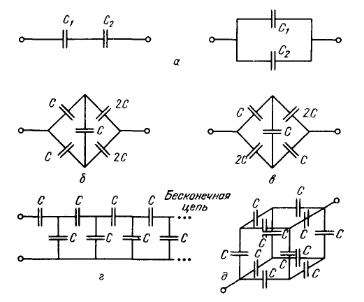
\includegraphics[scale=0.6]{d10_5_1.png}  
\end{center}

%%% Local Variables: 
%%% mode: latex
%%% TeX-master: "../../../report"
%%% End: 
